\documentclass{main.tex}[subfiles]
\begin{document}
\newpage
\section{Вычислительные эксперименты}
\subsection{Предобработка данных и выравнивание}

Фотографии были обработаны нейросетью, предварительно обученной на наборе изображений AngelinaDataset + DSBI.
% TODO tell how many photos are there?

Затем полученные тексты (запросы) и исходные тексты документов (референсы) прошли обработку, описанную в разделе \ref{subsection:preprocessing}, после чего было выполнено выравнивание.
Результаты выравнивания использованы для исправления .json-файлов, содержащих аннотациии (псевдометки).
Произведён подсчёт числа вхождений слов на каждой странице распознанного текста в словаре, составленном из слов исходного текста (до и после выравнивания).
Распределение доли слов, которые встречаются в исходном тексте, показано на рис. \ref{fig:frequencies}.

\begin{figure}[H]
    \centering
    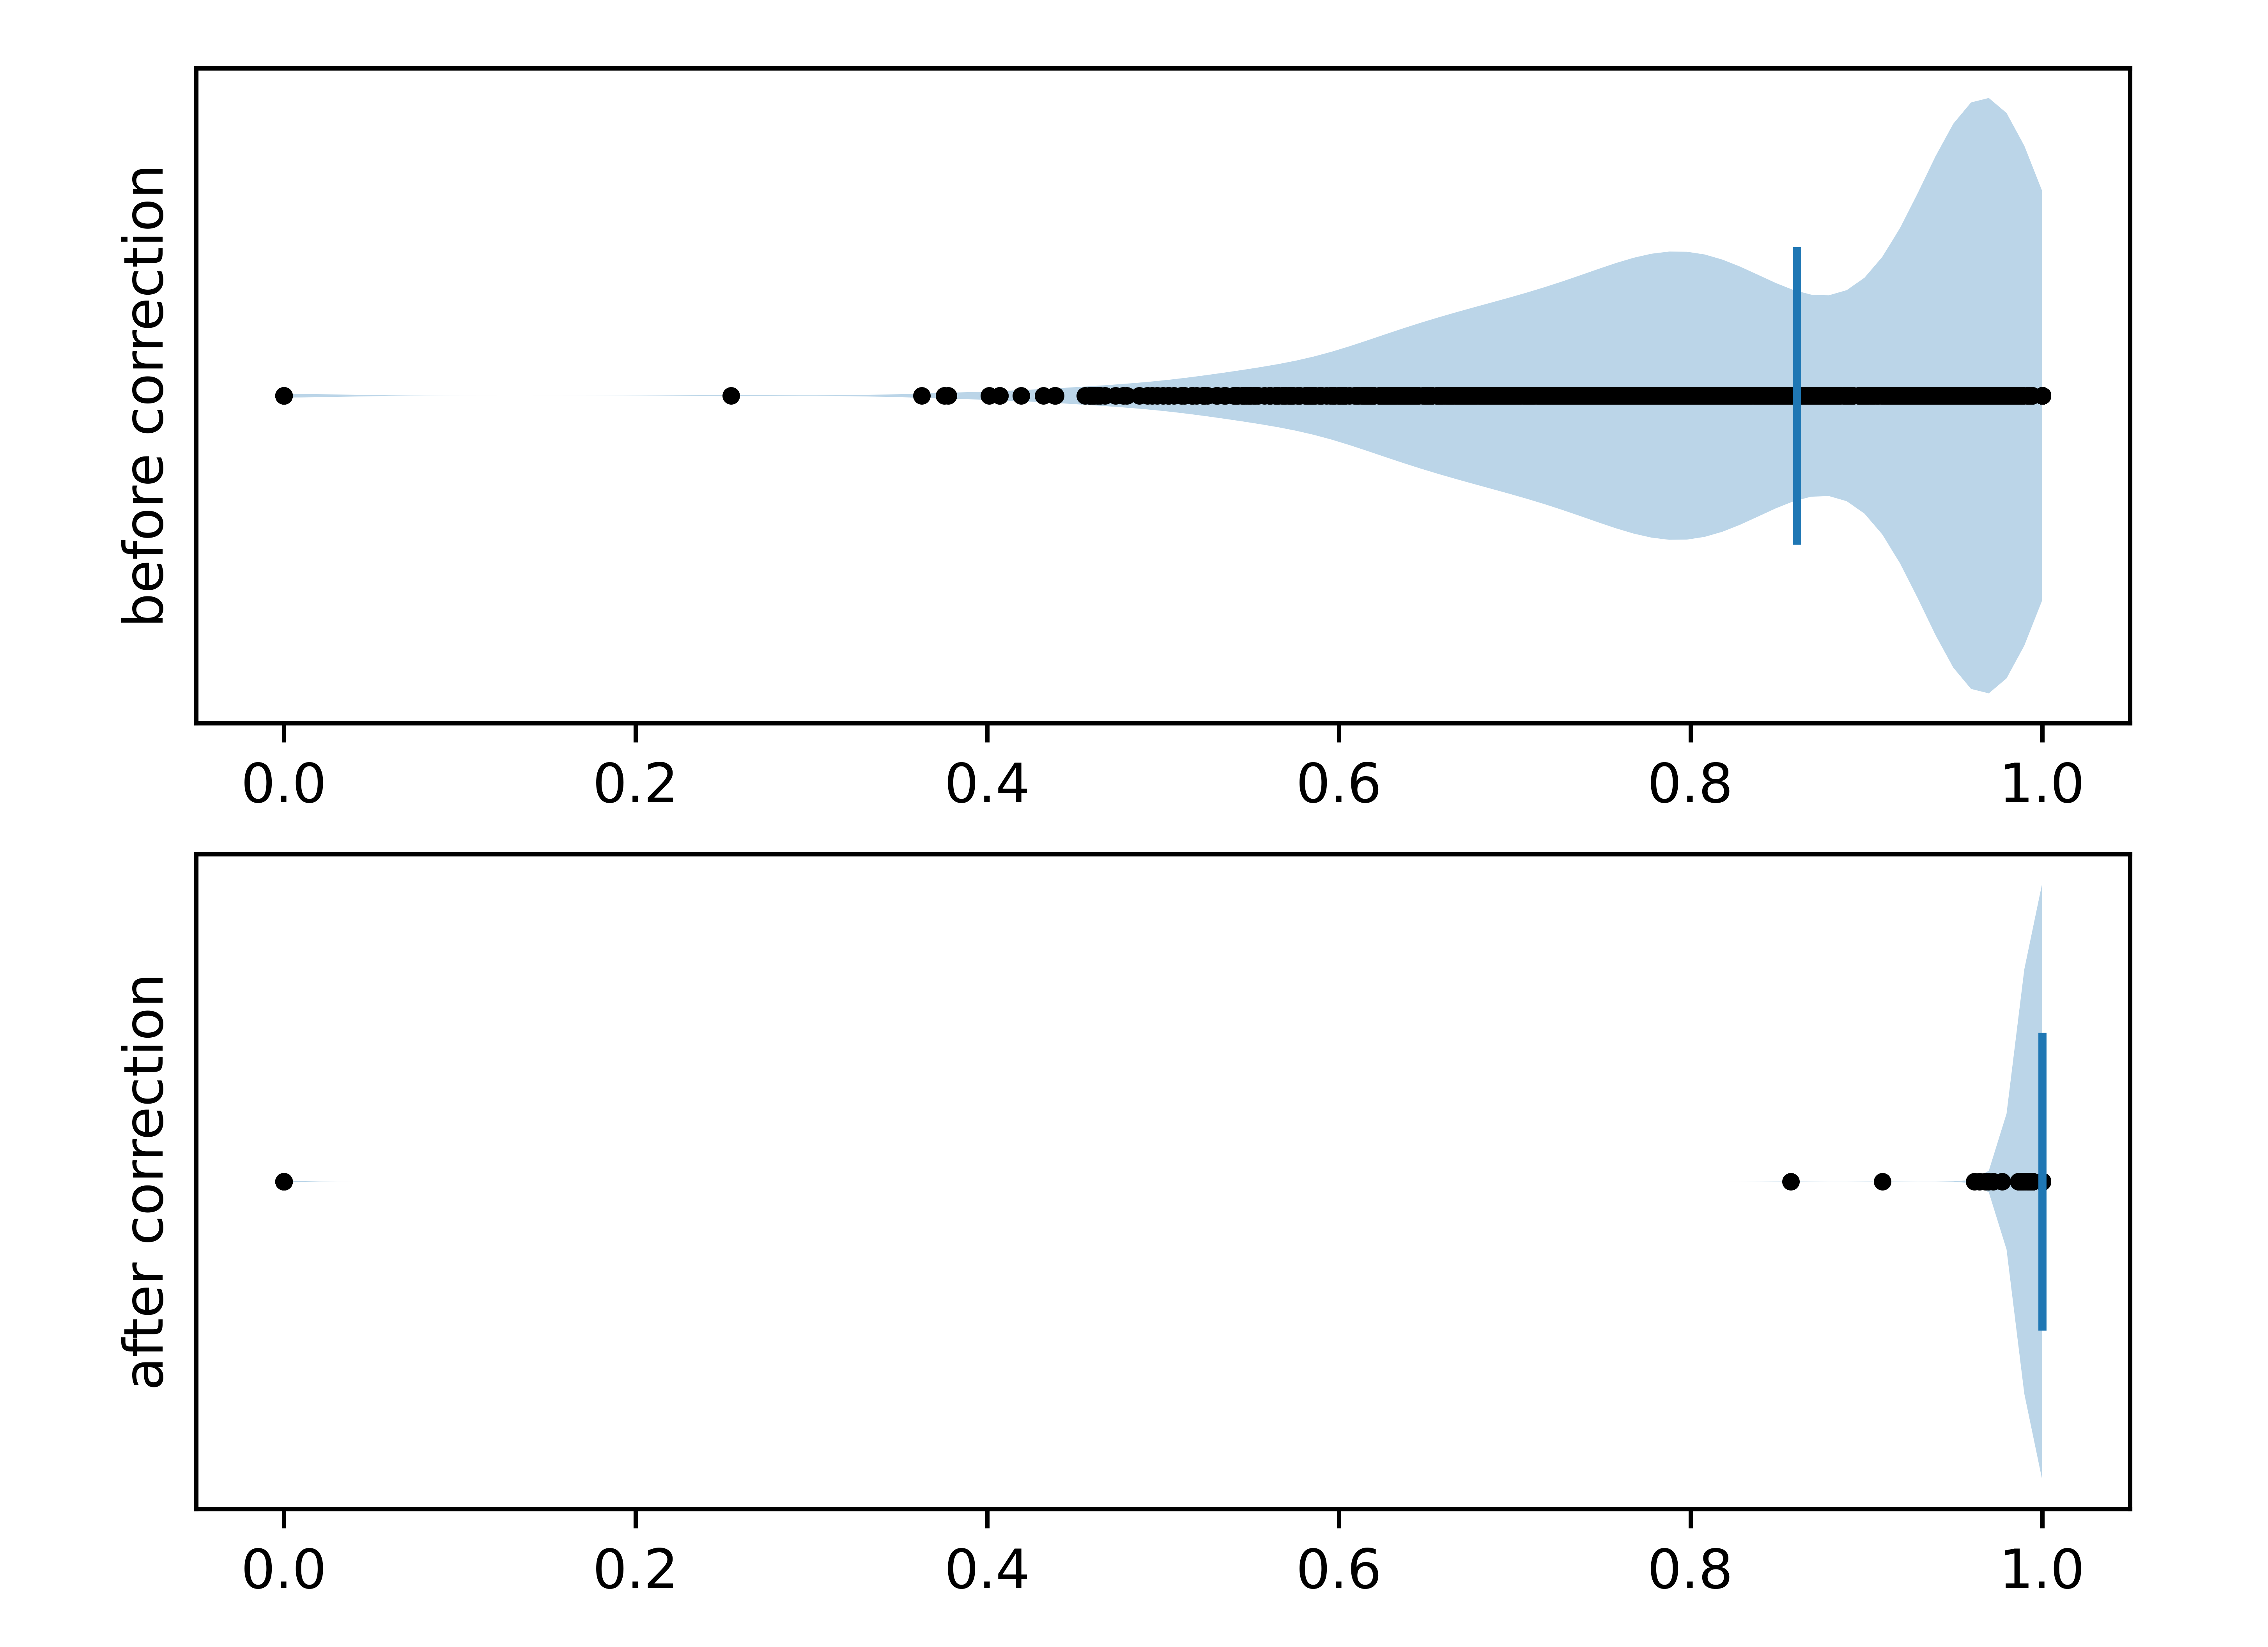
\includegraphics[width=\myPictWidth]{frequencies}
    \caption{Доля слов в распознанном тексте, встречающихся в исходном: до выравнивания (вверху) и после (внизу). Чёрные точки -- элементы выборки, голубая область -- ядерная оценка плотности распределения с ядром Гаусса (т. н. violinplot), синяя вертикальная черта -- медиана выборки}
    \label{fig:frequencies}
\end{figure}

\subsection{Обучение нейронной сети}

Произведено 6 запусков процесса обучения нейронной сети по 300 итераций: 3 раза с обучающим набором AngelinaDataset + DSBI и 3 раза с расширенным набором AngelinaDataset + DSBI + данные с исправленными псевдометками.
Используются только те страницы с псевдометками, в которых после исправления не встречаются слова, отсутствующие в референсной строке (1164 страницы, разделённые на тренировочную и валидационную выборку в пропорции 9:1).
Результаты сравнения качества моделей на валидационных, т. е. не используемых при обучении, долях выборок представлены в табл. \ref{table:validate_results}.
% TODO formulas: write about how the metrics are calculated, loss function
% TODO results: add SSL without labels correction

% latex table generated in R 4.0.5 by xtable 1.8-4 package
% Sat May 29 22:42:56 2021
\begin{table}[ht]
    \centering
    \caption{Показатели качества обученных моделей (среднее по 3 независимым повторам обучения)}
    \begin{tabular}{l p{.17\textwidth} rrr}
        \hline
        валидационный набор & обучение на расширенном наборе & точность & полнота & $F_1$-мера \\
        \hline
        \multirow{2}{*}{ Книги (AngelinaDataset) }
         & нет & 0.998 & 0.997 & 0.998 \\
         & да  & 0.996 & 0.994 & 0.995 \\
        \multirow{2}{*}{ Рукописи (AngelinaDataset) }
         & нет & 0.997 & 0.997 & 0.997 \\
         & да  & 0.992 & 0.990 & 0.991 \\
        \multirow{2}{*}{ DSBI }
         & нет & 0.997 & 0.995 & 0.996 \\
         & да & 0.986 & 0.989 & 0.987 \\
        \multirow{2}{*}{ Книги с псевдометками }
         & нет & 0.817 & 0.111 & 0.194 \\
         & да & 0.982 & 0.989 & 0.986 \\
        \hline
    \end{tabular}
    \label{table:validate_results}
\end{table}


\end{document}